\subsection{Confusion matrix}
\begin{wrapfigure}{l}{0.6\textwidth}
	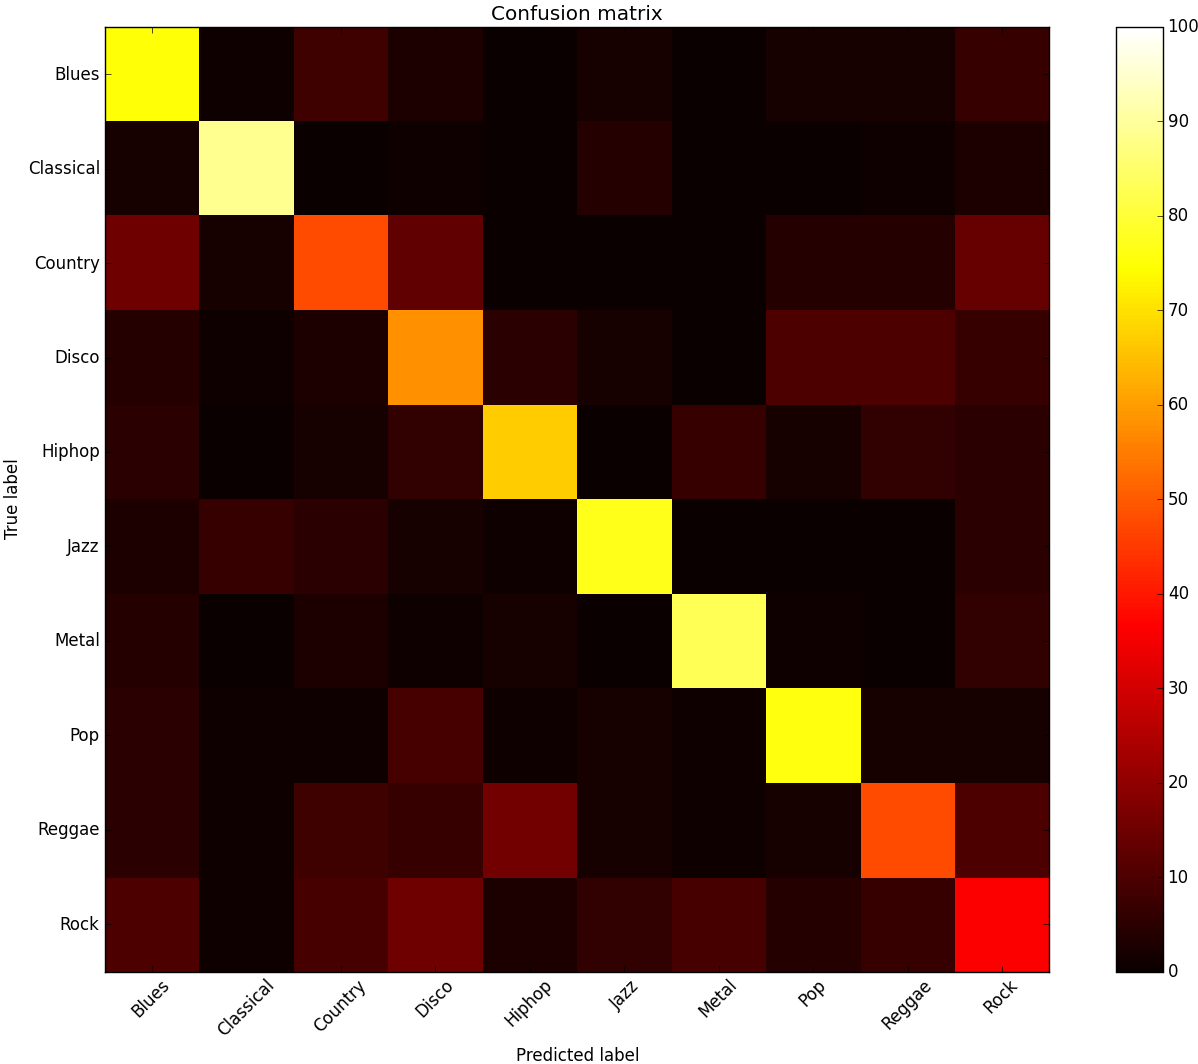
\includegraphics[width=\textwidth]{confusion_matrix.png}
	\caption{Confusion matrix of 10-fold CV predictions and true labels, white is 100\% accuracy, black is 0\%}
	\label{fig:confusion}
\end{wrapfigure}
The confusion matrix in \ref{fig:confusion} is built from MFCC+HCDF Fisher Vector feature set with KNN5 classifier. We see that Classical, Metal , Blues and Jazz are the best identified genres, with accuracy exceeding 70\%, this corroborates with our visualization in \ref{fig:tsne1} which showed clear clustering for those genres. Genre pairs with the most confusion are \{Reggae, Hip-Hop\}, \{Rock, Disco\}, \{Rock, Country\}, which also corroborates with our visualizations in \ref{fig:tsne2}. 
\subsection{Classifiers and features}
It is no surprise that the best single classifier before ensemble learning is linear SVM, because our underlying features are represented in Fisher Vectors, which lends itself to efficient linear classification.
The Fisher Kernel inherits advantages from both generative and discriminative models by building a kernel from a generative model (GMM).
